\documentclass[11pt]{article}
\usepackage[margin=1in]{geometry}
\usepackage{graphicx}
\usepackage{hyperref}
\usepackage{enumitem}
\usepackage{booktabs}
\usepackage{xcolor}
\usepackage{subcaption}

\title{Camera Accuracy Notes}
\author{Aditya Bondada}
\date{\today}

\begin{document}
\maketitle

\section{Current Issues}

\begin{enumerate}
    \item Sample being stuck to the suction cup after turning off the ePick vacuum.
    \item Robot move to Tag 0 always fails (has an offset to the tag).
\end{enumerate}

\begin{figure}[h]
    \centering
    \begin{subfigure}[b]{0.48\textwidth}
        \centering
        \includegraphics[width=\textwidth]{../images/tag0_offset.png}
        \caption{tag0\_offset}
    \end{subfigure}
    \hfill
    \begin{subfigure}[b]{0.48\textwidth}
        \centering
        \includegraphics[width=\textwidth]{../images/tag0_newpos.png}
        \caption{tag0\_newpos}
    \end{subfigure}
    \label{fig:tag0_comparison}
\end{figure}

\begin{figure}[h]
    \centering
    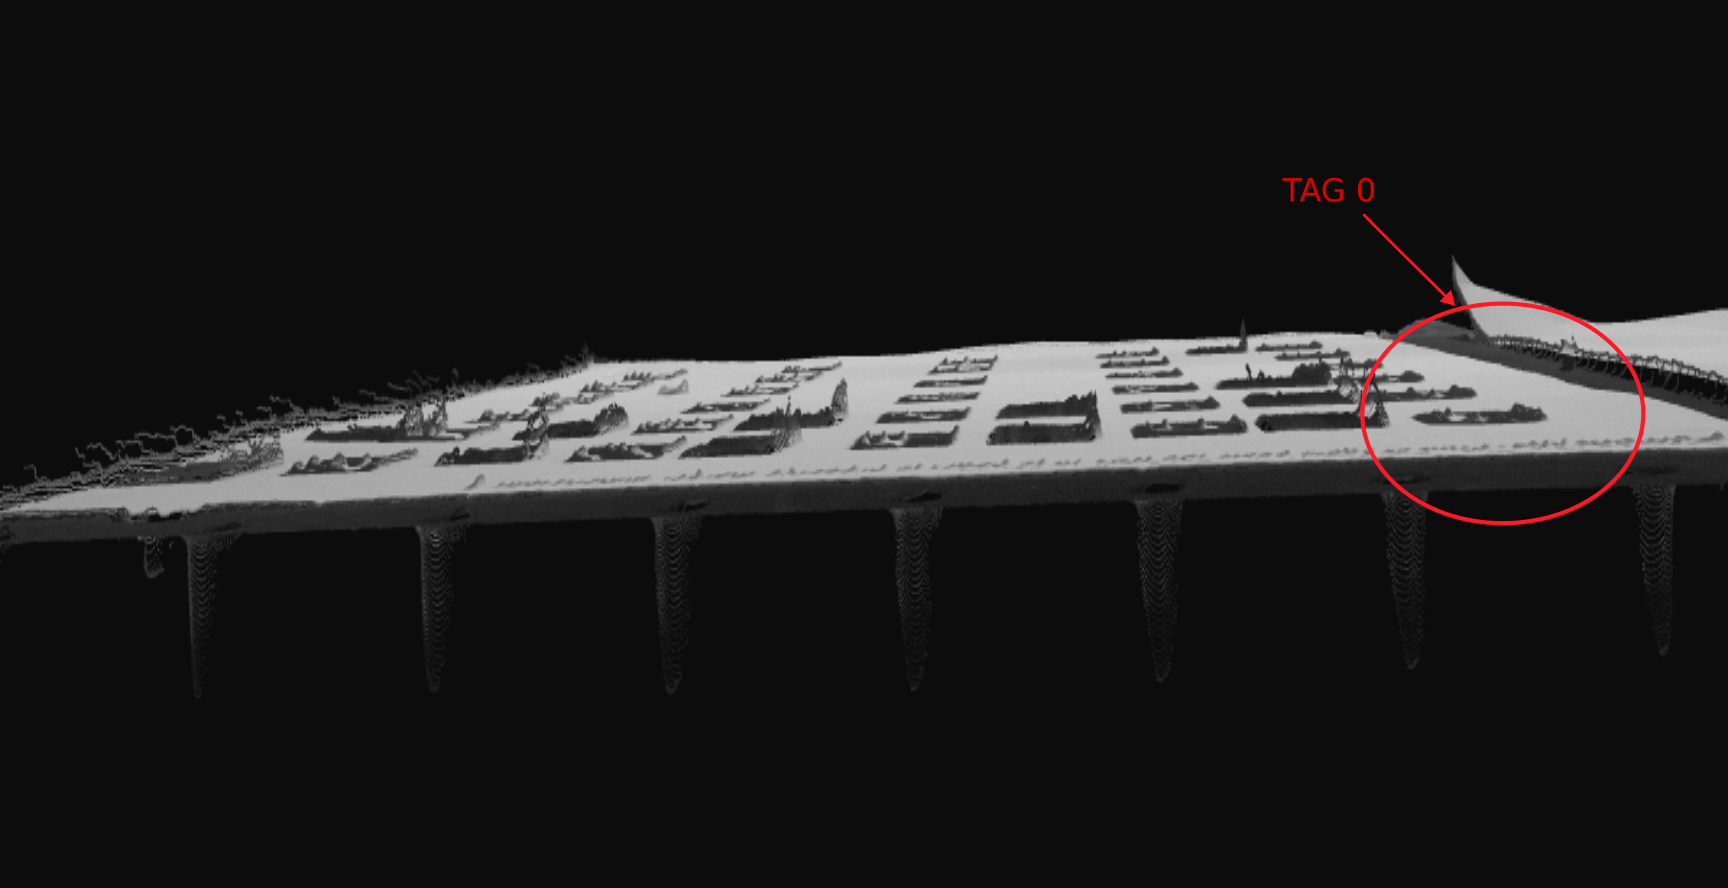
\includegraphics[width=0.9\textwidth]{../images/tag0_depth.png}
    \caption{3D point cloud view highlighting Tag 0 location on a raised/angled surface at the edge of the hotplate.}
    \label{fig:tag0_depth}
\end{figure}

\begin{figure}[h]
    \centering
    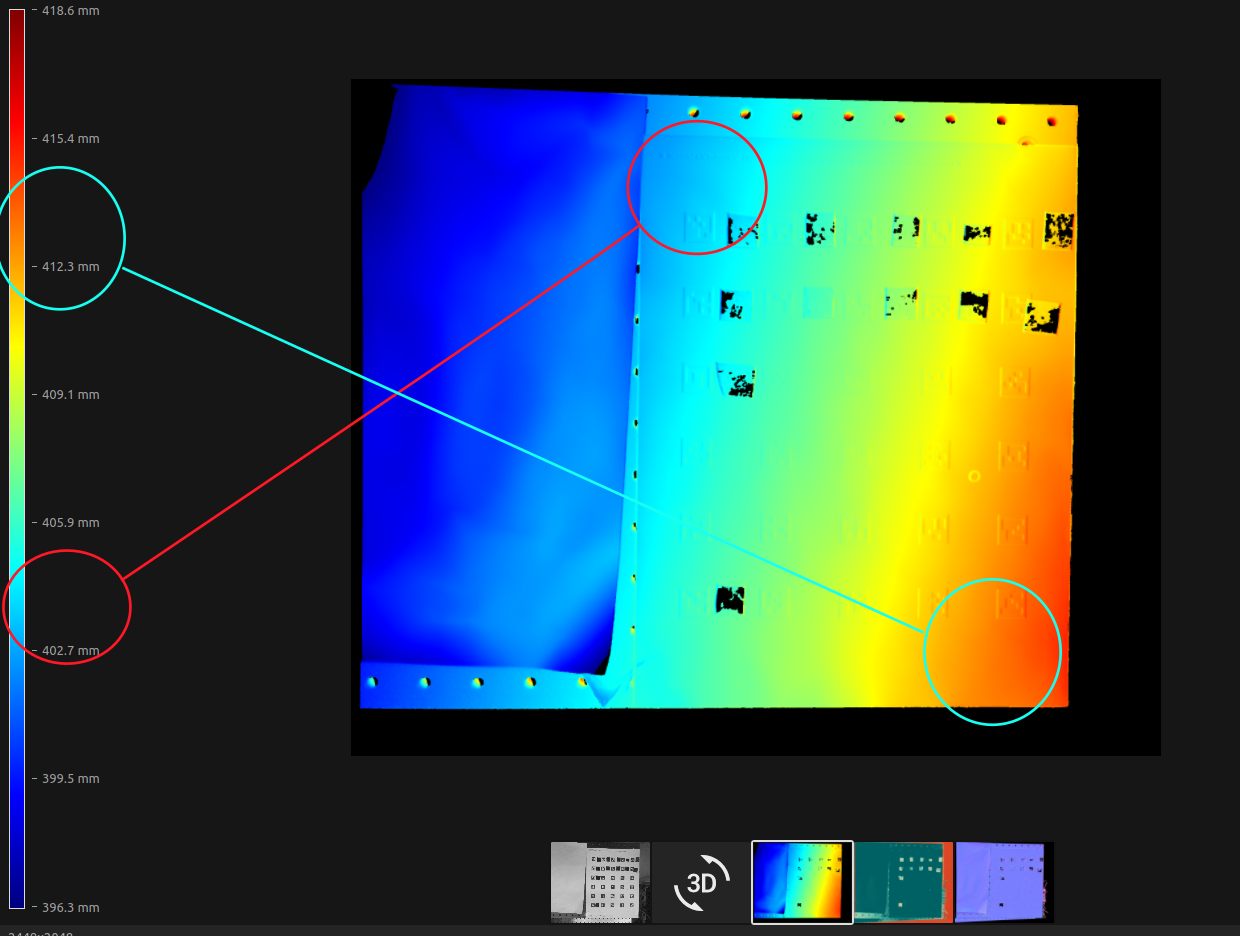
\includegraphics[width=0.9\textwidth]{../images/depth_map_aruco_edited.png}
    \caption{Zivid depth map showing ArUco markers on the hotplate setup.}
    \label{fig:depth_map_aruco}
\end{figure}

\begin{figure}[h]
    \centering
    \includegraphics[width=0.9\textwidth]{../images/robot_TCP_highlighted.png}
    \caption{Robot TCP highlighted.}
    \label{fig:robot_tcp}
\end{figure}

\begin{figure}[h]
    \centering
    \begin{subfigure}[b]{0.32\textwidth}
        \centering
        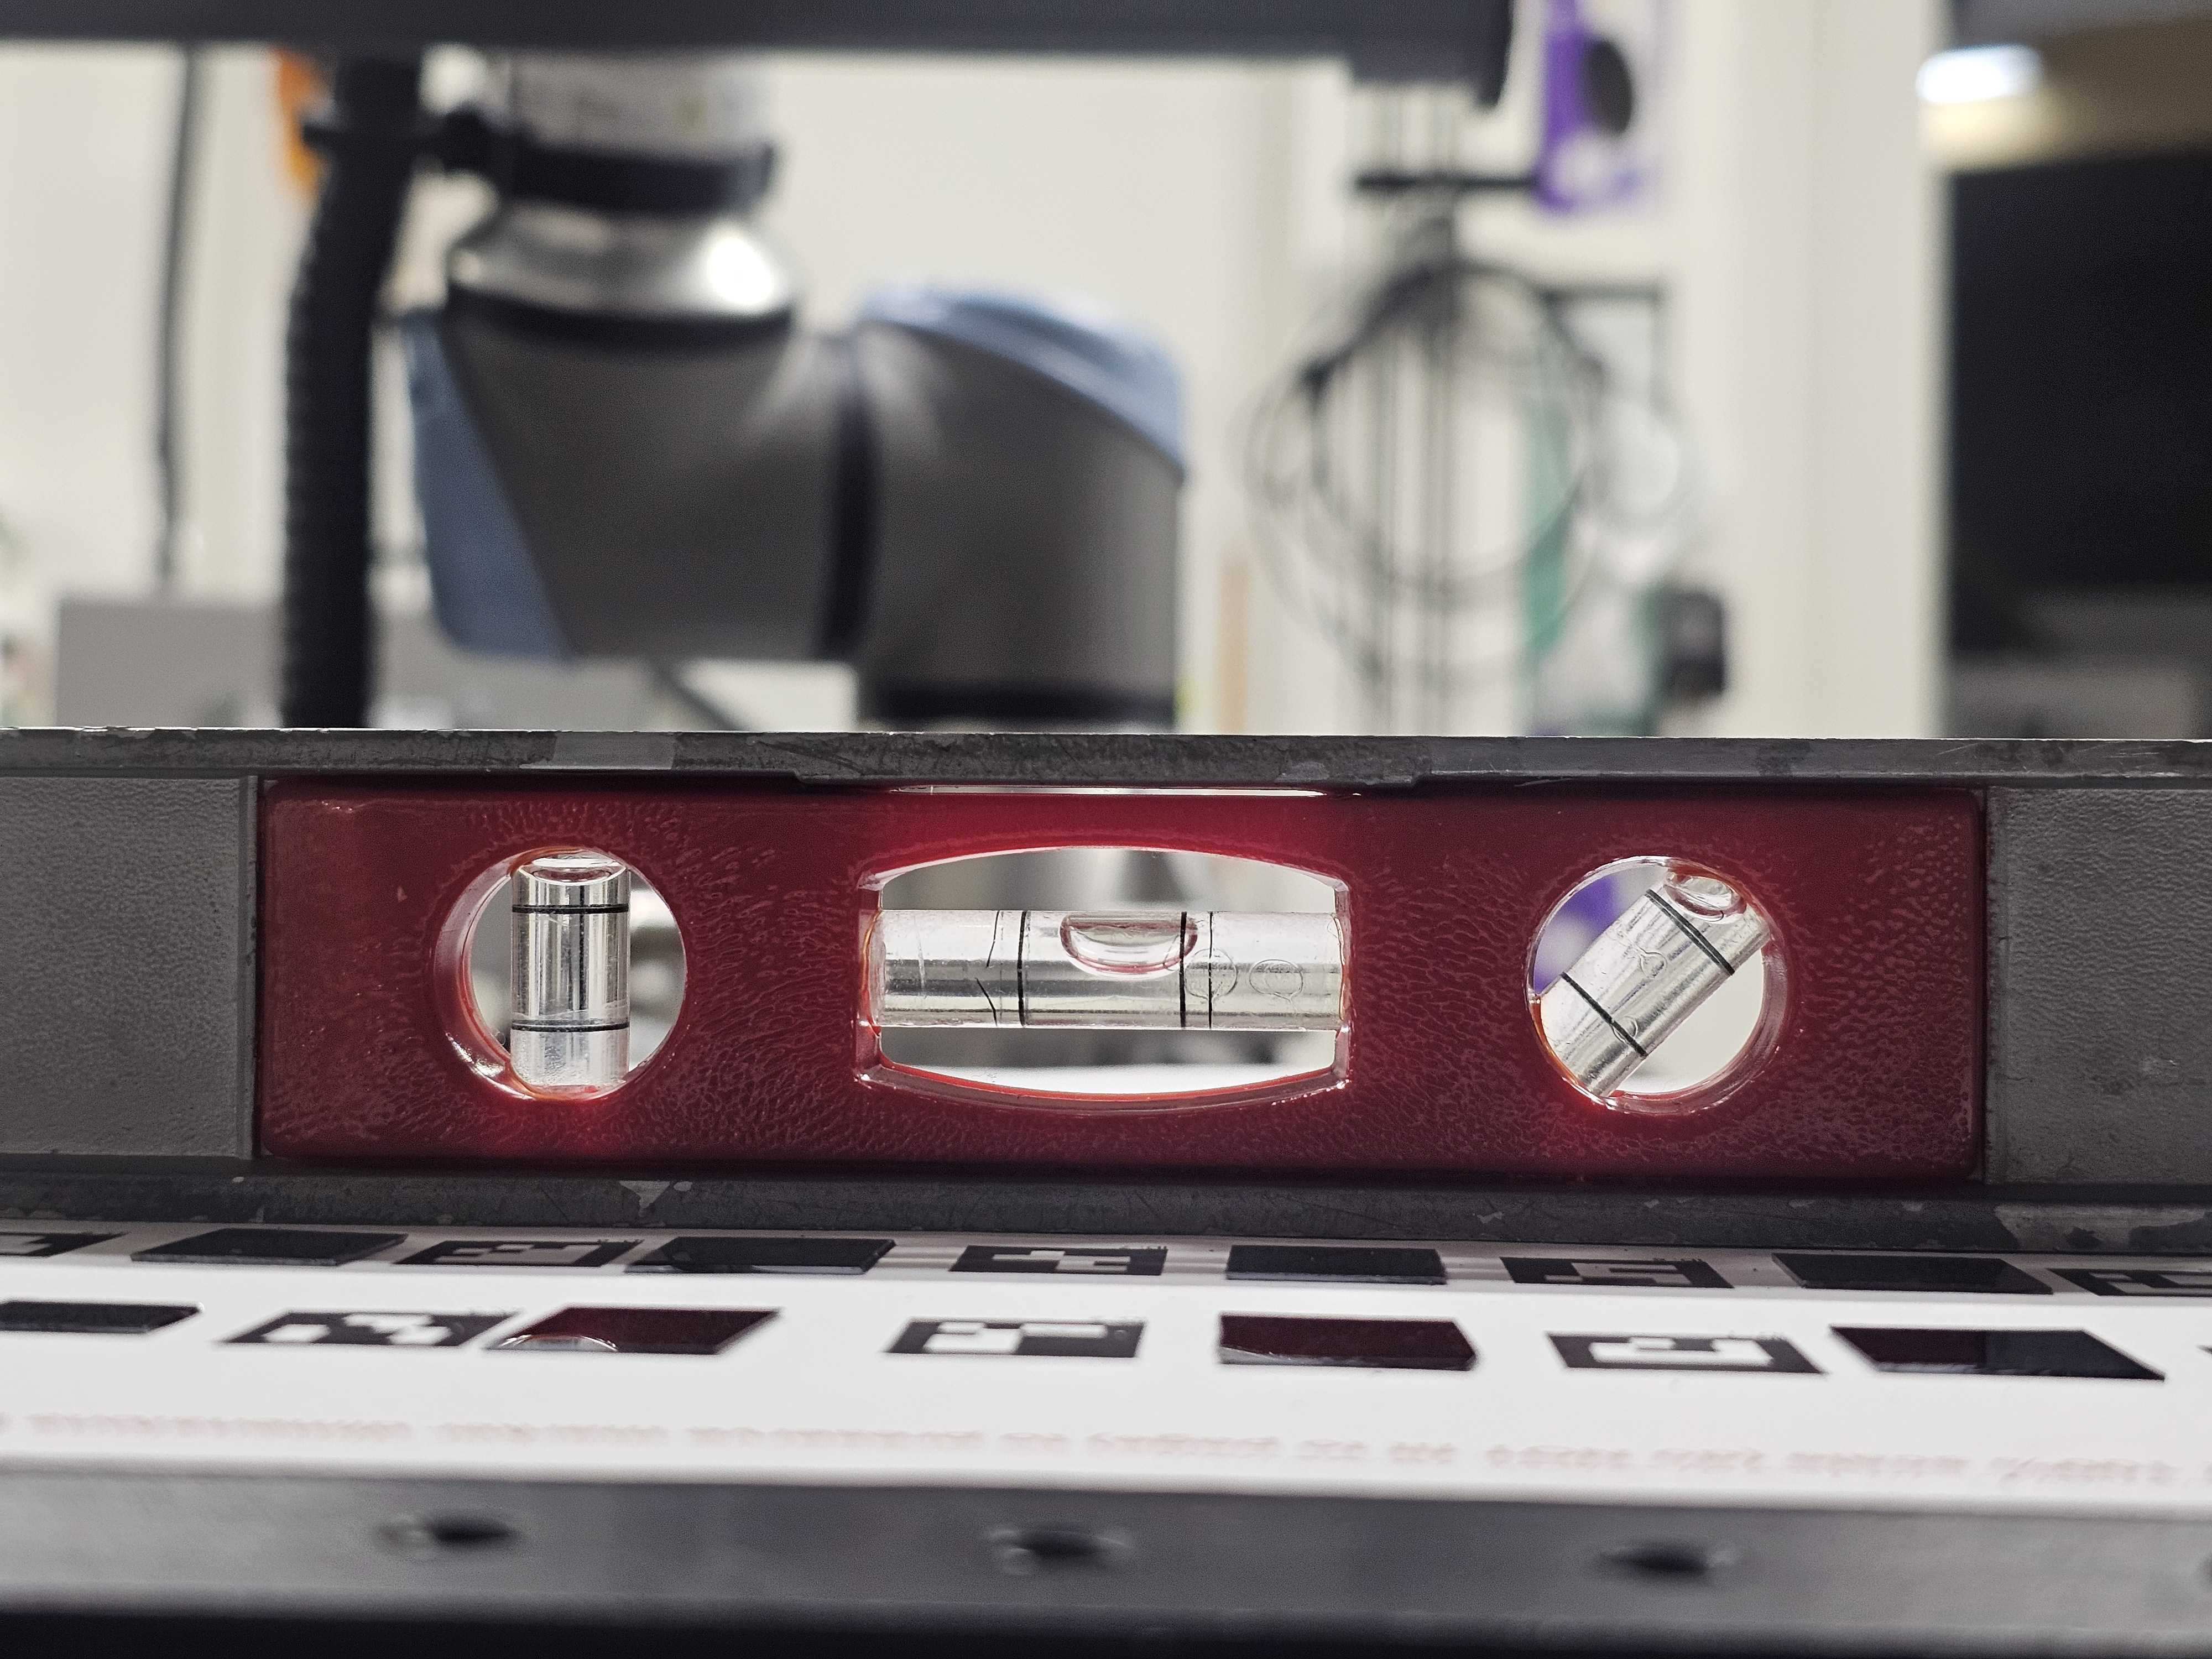
\includegraphics[width=\textwidth]{../images/tag_flat.jpg}
        \caption{tag\_flat}
    \end{subfigure}
    \hfill
    \begin{subfigure}[b]{0.32\textwidth}
        \centering
        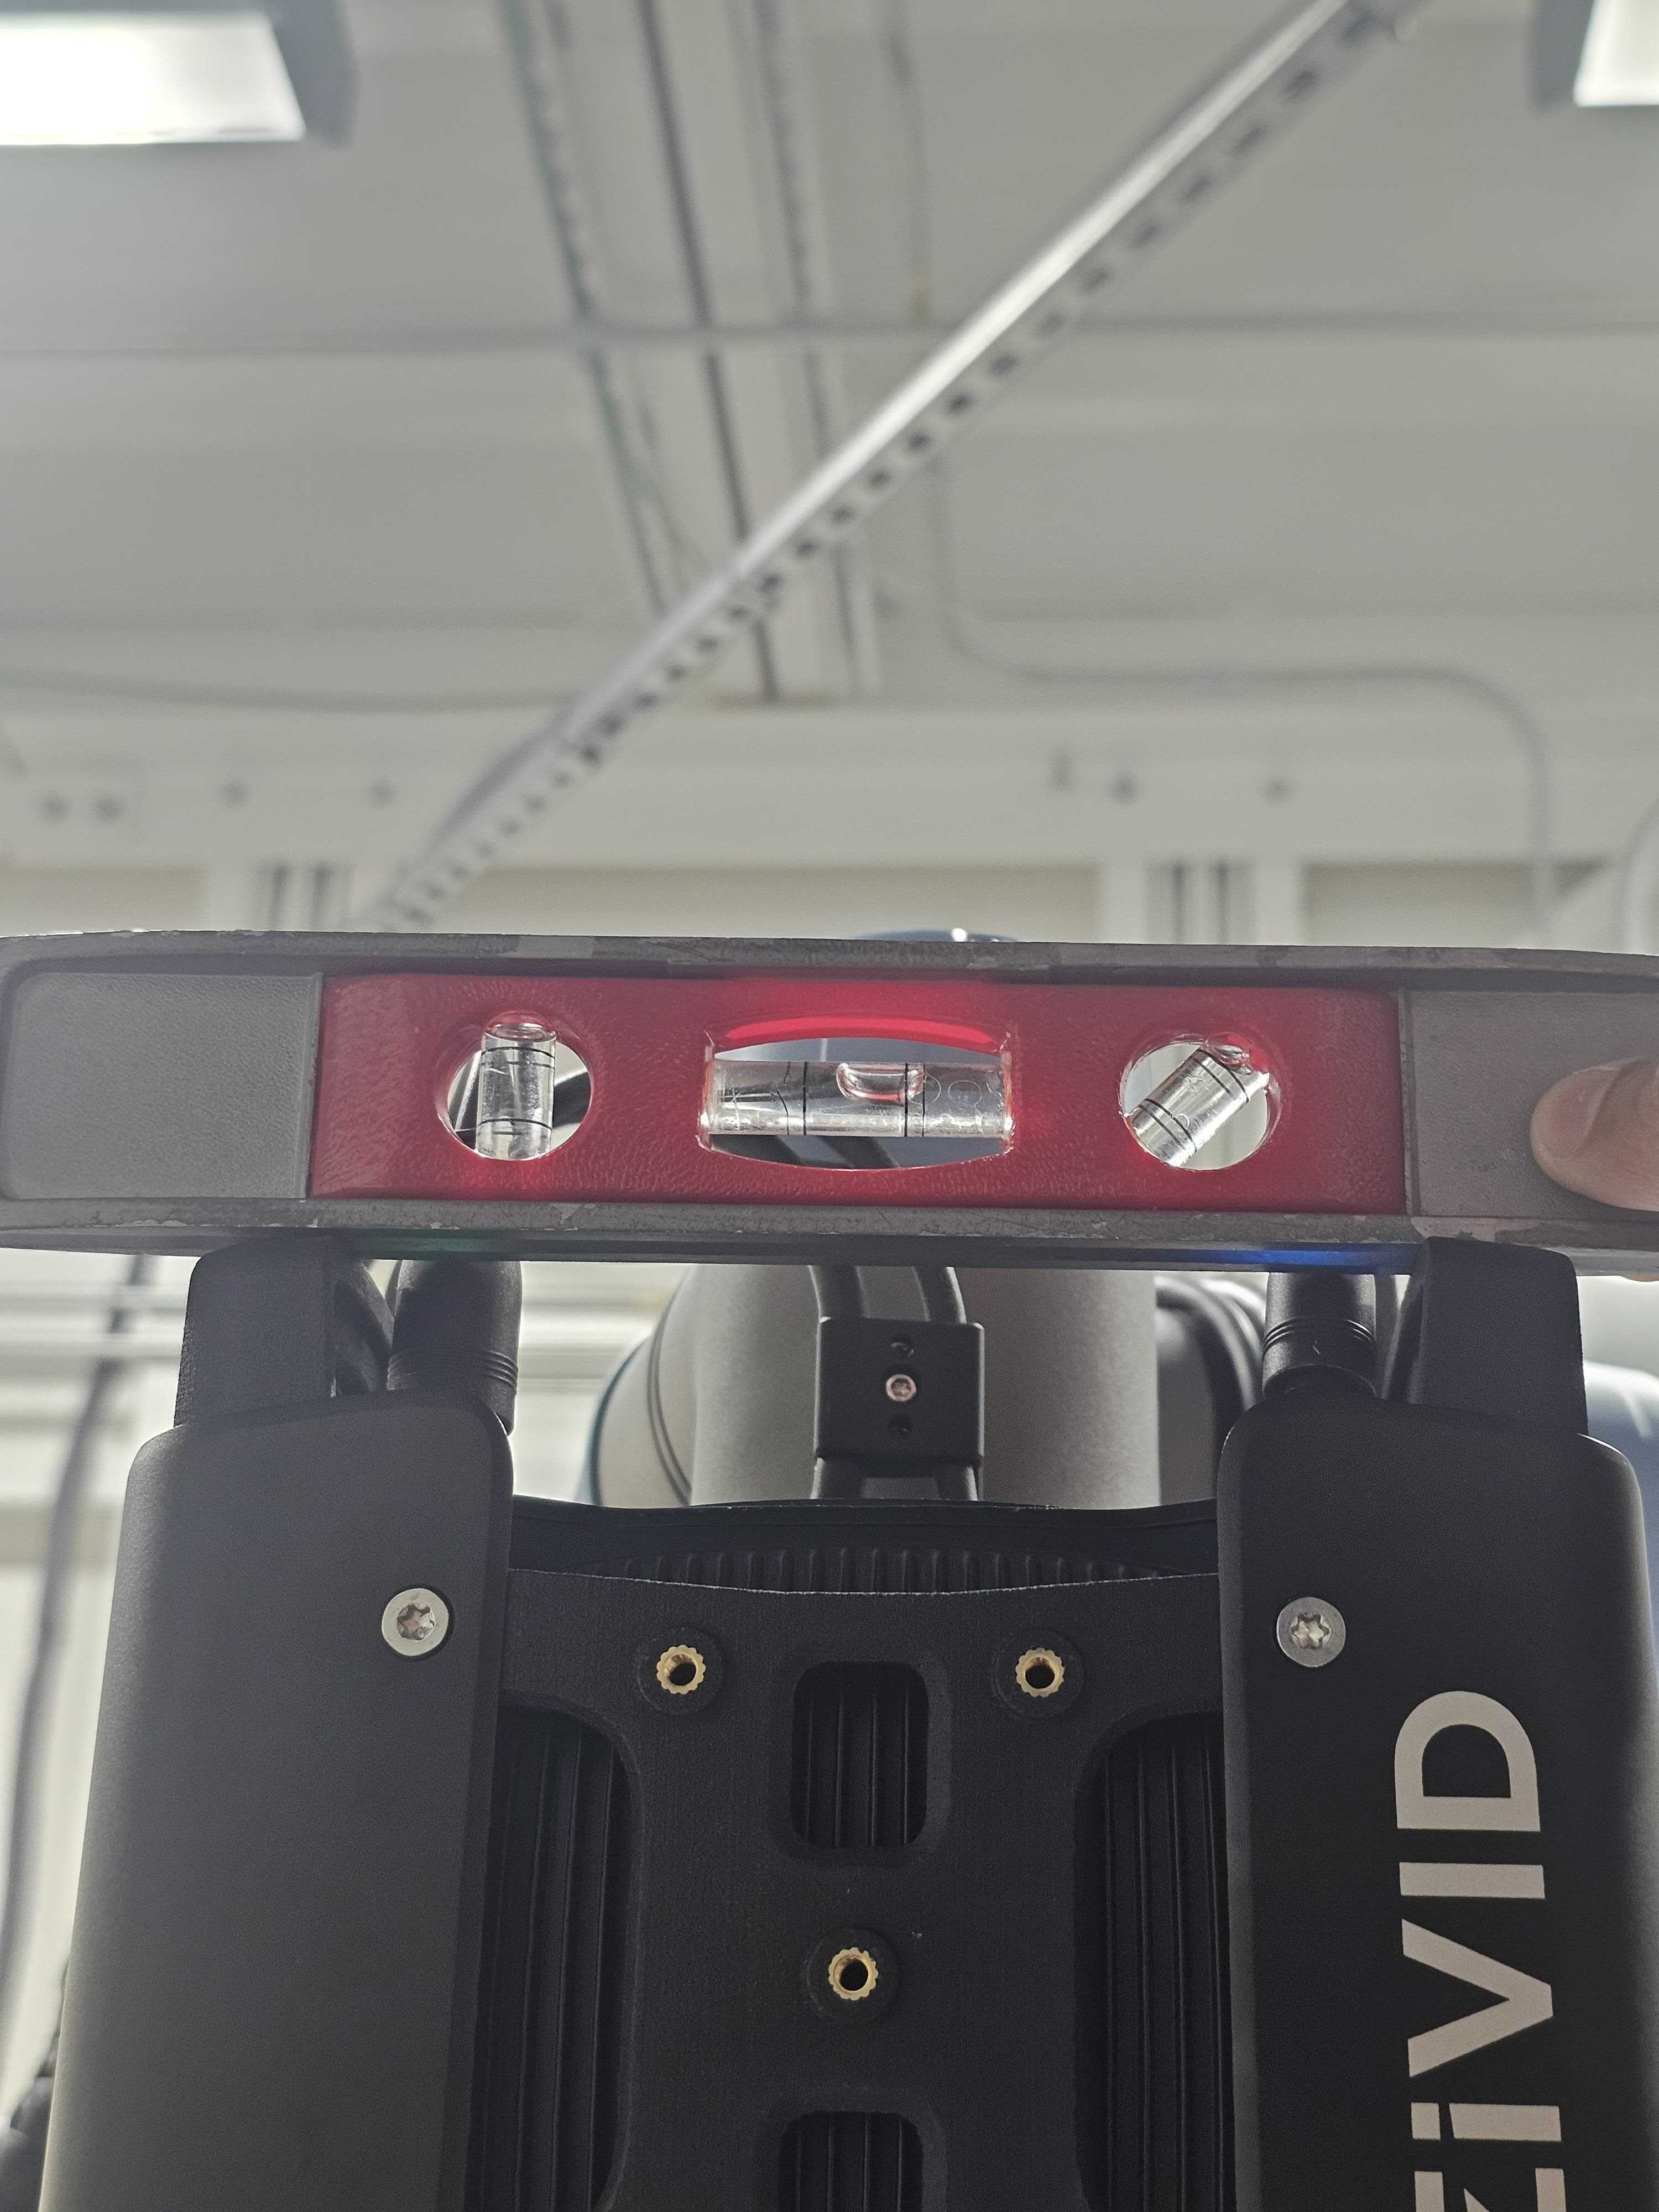
\includegraphics[width=\textwidth]{../images/camera_flat.jpg}
        \caption{camera\_flat}
    \end{subfigure}
    \hfill
    \begin{subfigure}[b]{0.32\textwidth}
        \centering
        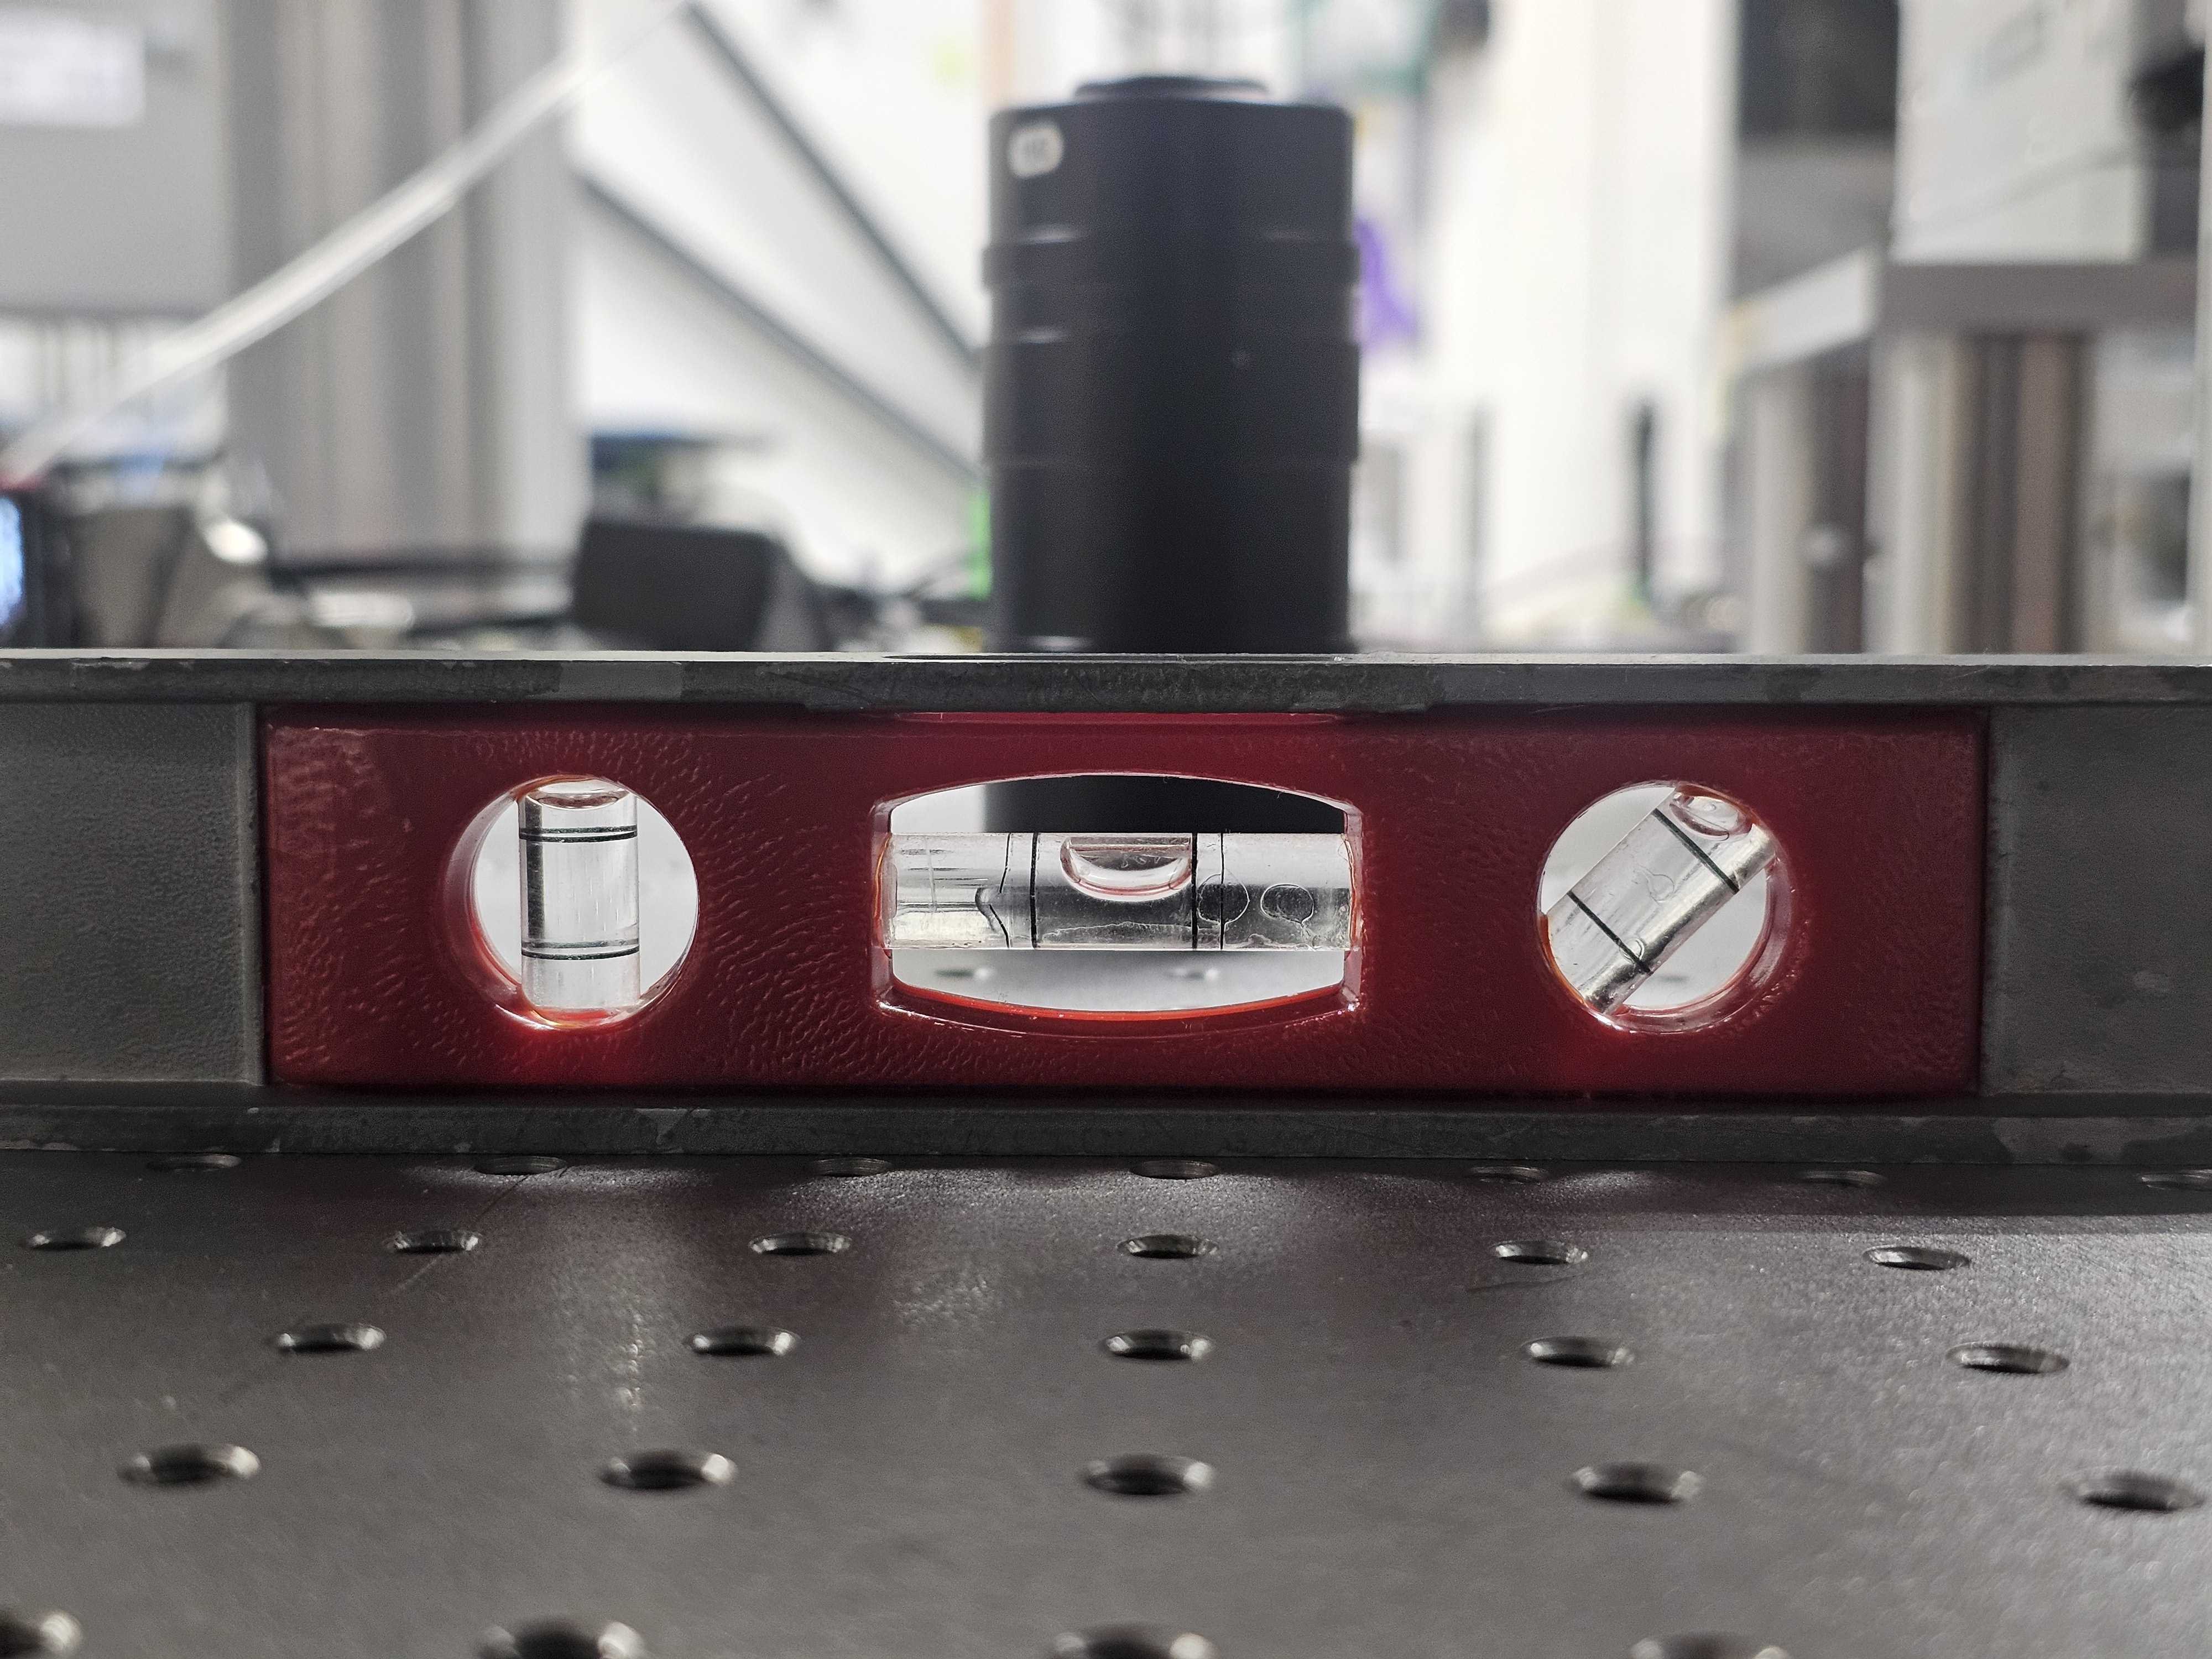
\includegraphics[width=\textwidth]{../images/table_flat.jpg}
        \caption{table\_flat}
    \end{subfigure}
    \label{fig:flat_views}
\end{figure}

\end{document}
